\documentclass{article}
\usepackage{amsmath, tikz, cancel}
\usetikzlibrary{automata, positioning, arrows}

\begin{document}

\textbf{Exercise 1}. Let $\Sigma$ be the alphabet $\{a, b\}$. Consider the grammar $G =
(\Sigma, \{S, A\}, S, P)$ where $P$ contains the following rules:\\
\begin{center}
$S \rightarrow AA, \hspace{0.5cm} S \rightarrow a, \hspace{0.5cm} S \rightarrow SA, \hspace{0.5cm} A \rightarrow ab$.\\
\end{center}
(i) Justify that $G$ is context-free.\\
(ii) Construct a PDA that recognizes $L(G)$. \\

\textbf{ANSWER:}

i) $G$ is context free because of the nature of the left side of each production rule. Because each rule is agnostic to the surrounding context of the word it is in, it the grammar is a context-free grammar. If it weren't, then we could have rules such as $aS \rightarrow Sa$, which would consume an a in the word, which inherently relies on the context of the word around it. \\

ii) In order to convert the CFG to a PDA, we convert $G$ to $G'$. This modification involves changing the production rules to include symbols, and making new rules that convert these new symbols into their original letters. That way, the construction of the PDA is straightforward. 
$G' := (\Sigma, \{S, A, V_a, V_b\}, S, P')$, where $P'$ is defined by:
\begin{center}
	$S \rightarrow AA, \hspace{0.5cm} S \rightarrow V_a, \hspace{0.5cm} S \rightarrow SA, \hspace{0.5cm} A \rightarrow V_aV_b$.\\
	$V_a \rightarrow a, \hspace{0.5cm} V_b \rightarrow b$. \\
\end{center}

We then construct the PDA using these new rules. Any instance of an original letter being said will now be replaced by pushing the appropriate symbol onto the stack, and only by popping it can we say the original letter. The following PDA is as follows:

\begin{center}
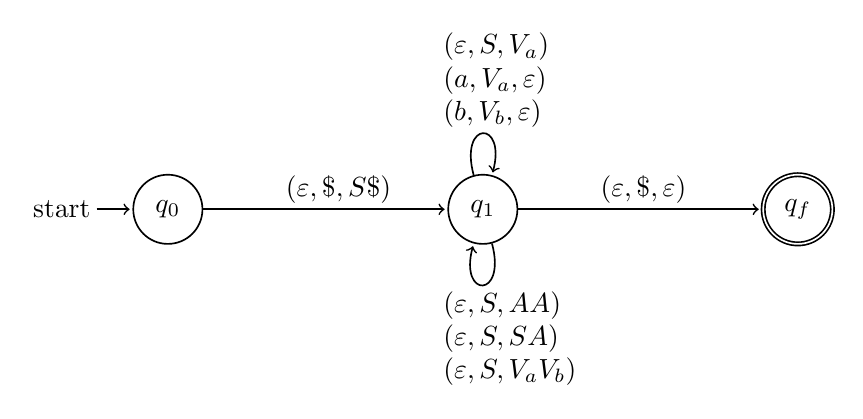
\begin{tikzpicture}
[->,shorten >=1pt, auto,node distance=4cm,on grid,semithick,inner sep=2pt,bend angle=45]

\node[state, initial] (q0) {$q_0$};
\node[state, right of=q0] (q1) {$q_1$};
\node[state, accepting, right of=q1] (qf) {$q_f$};

\path[->]
	(q0) edge node [text width=1cm] {$(\varepsilon, \$, S\$)$} (q1)
	(q1) edge [loop above] node [text width=1cm] {$(\varepsilon, S, V_a)$
												 $(a, V_a, \varepsilon)$
												 $(b, V_b, \varepsilon)$} ()
		edge [loop below] node [text width=1cm] {$(\varepsilon, S, AA)$
												$(\varepsilon, S, SA)$ 
												$(\varepsilon, S, V_aV_b)$}()
		edge node [text width=1cm] {$(\varepsilon, \$, \varepsilon)$} (qf);
\end{tikzpicture}
\end{center}


\textbf{Exercise 2}. Let $\Sigma$ be the alphabet $\{a, b\}$. Consider the following PDA $\mathcal{A}$
over $\Sigma$ whose stack alphabet is $\Gamma = \{\$, W, Z, X, Y \}$ (where the starting stack
symbol is $\$$)

(This is where the PDA would go :) But you know it and I know it so let's pretend its here instead)

Write a grammar that generates $L(\mathcal{A})$. To do so, use the technique seen in
class, but remember to trim the resulting grammar as it will contains a lot of
useless variables and rules. (Trim as you go, or at the very end, that is up to
you.)\\

\textbf{ANSWER:}

To generate a CFG out of a PDA, we first need to ensure that the original PDA has transitions that either increase or decrease the stack size, and a final state led to by only one transition. Luckily, we have both, so we can begin enumerating the possible rules. They're created through tuples of $Q \times Q \times \Gamma$. Now we create a CFG $G'$ that is as follows: $G' := (\Sigma, \{Q \times Q \times \Gamma\}, (i, f, \$), P')$ with $P'$ defined by: (To save time, no transitions will be shown that start with $f$, or end with $i$, as these are impossible given the nature of the original PDA).

\begin{center}
	$(q, q, X) \rightarrow a$ \\
	$(q, q, Y) \rightarrow b$ \\
	$(q, q, Z) \rightarrow a$ \\
	$(q, q_f, \$) \rightarrow \varepsilon$ \\
	\hfill \break
	$(i, q, \$) \rightarrow (q, q, Z)(q, q, \$)$ \\ 
	$(i, q_f, \$) \rightarrow (q, q, Z)(q, q_f, \$)$ \\
	\hfill \break
	$(q, q, Z) \rightarrow (q, q, W)(q, q, W)$ \\
	$(q, q_f, Z) \rightarrow (q, q, W)(q, q_f, W)$ \\
	\hfill \break
	$(q, q, W) \rightarrow (q, q, Z)(q, q, W)$ \\
	$(q, q_f, W) \rightarrow (q, q, Z)(q, q_f, W)$ \\
	\hfill \break
	$(q, q, W) \rightarrow (q, q, X)(q, q, Y)$ \\
	$(q, q_f, W) \rightarrow (q, q, X)(q, q_f, Y)$ \\
\end{center}

We can trim the list here to only include reachable sets of states. Any state has a triple that begins with $q_f$ can be immediately removed. If any triple involves a transition not reflected in the original PDA, we can remove that as well. The states we remove are as follows (marked by an \textbf{X}). 

\begin{center}
	$(q, q, X) \rightarrow a$ \\
	$(q, q, Y) \rightarrow b$ \\
	$(q, q, Z) \rightarrow a$ \\
	$(q, q_f, \$) \rightarrow \varepsilon$ \\
	\hfill \break
	$(i, q, \$) \rightarrow (q, q, Z)(q, q, \$)$ \textbf{X} \\ 
	$(i, q_f, \$) \rightarrow (q, q, Z)(q, q_f, \$)$ \\
	\hfill \break
	$(q, q, Z) \rightarrow (q, q, W)(q, q, W)$ \\
    $(q, q_f, Z) \rightarrow (q, q, W)(q, q_f, W)$ \textbf{X} \\
	\hfill \break
    $(q, q, W) \rightarrow (q, q, Z)(q, q, W)$ \\
    $(q, q_f, W) \rightarrow (q, q, Z)(q, q_f, W)$ \textbf{X} \\
	\hfill \break
    $(q, q, W) \rightarrow (q, q, X)(q, q, Y)$ \\
    $(q, q_f, W) \rightarrow (q, q, X)(q, q_f, Y)$ \textbf{X} \\
\end{center}

Leaving us with:

\begin{center}
	$(q, q, X) \rightarrow a$ \\
	$(q, q, Y) \rightarrow b$ \\
	$(q, q, Z) \rightarrow a$ \\
	$(q, q_f, \$) \rightarrow \varepsilon$ \\
	$(i, q_f, \$) \rightarrow (q, q, Z)(q, q_f, \$)$ \\ 
	$(q, q, Z) \rightarrow (q, q, W)(q, q, W)$ \\
	$(q, q, W) \rightarrow (q, q, Z)(q, q, W)$ \\
	$(q, q, W) \rightarrow (q, q, X)(q, q, Y)$ \\
\end{center}

For $P'$. We can convert the tuples to similar stack symbols, and get the grammar: 

\begin{center}
	$X \rightarrow a$ \\
	$Y \rightarrow b$ \\
	$Z \rightarrow a$ \\
	$E \rightarrow \varepsilon$ \\
	$S \rightarrow ZE$ \\ 
	$Z \rightarrow WW$ \\
	$W \rightarrow ZW$ \\
	$W \rightarrow XY$ \\
\end{center}


\textbf{Exercise 3}. Let $\Sigma$ be the alphabet $\{a, b\}$.  Consider the grammar $G =
(\Sigma, \{S, A\}, S, P)$ where $P$ contains the following rules:\\
\begin{center}
$S \rightarrow aB,\hspace{0.5cm} S \rightarrow bA, \hspace{0.5cm} S \rightarrow \varepsilon$\\
$A \rightarrow aS,\hspace{0.5cm} A \rightarrow Sa$\\
$B \rightarrow bS,\hspace{0.5cm} B \rightarrow Sb$\\
\end{center}

(i) Describe the language generated by the grammar $G$.

(ii) Construct a PDA that recognizes $L(G)$.\\

\textbf{ANSWER:}

The language described by $G$ is $L = \{w\in\Sigma^* \mid n_a(w) = n_b(w)\}$ where $\Sigma = \{a, b\}$

To convert $G$ to a PDA, we must first convert $G$ to $G'$ in a similar manner to Problem 1. 

$G' := (\Sigma, \{S, V_a, V_b\}, S, P')$ where $P'$ is defined by:

\begin{center}
	$S \rightarrow V_aB, \hspace{0.5cm} S \rightarrow V_bA, \hspace{0.5cm} S \rightarrow \varepsilon$.\\
	$A \rightarrow V_aS \hspace{0.5cm} A \rightarrow SV_a$ \\
	$B \rightarrow V_bS \hspace{0.5cm} B\rightarrow SV_b$ \\
	$V_a \rightarrow a, \hspace{0.5cm}, V_b \rightarrow b$ \\
\end{center}

We then construct the PDA using these new rules. Any instance of an original letter being said will now be replaced by pushing the appropriate symbol onto the stack, and only by popping it can we say the original letter. The following PDA is as follows:

\begin{center}
	\begin{tikzpicture}
		[->,shorten >=1pt, auto,node distance=4cm,on grid,semithick,inner sep=2pt,bend angle=45]
		
		\node[state, initial] (i) {$i$};
		\node[state, right of=q0] (q) {$q$};
		\node[state, accepting, right of=q1] (f) {$f$};
		
		\path[->]
		(i) edge node [text width=1cm] {$(\varepsilon, \$, S\$)$} (q)
		(q) edge [loop above] node [text width=1cm] {$(\varepsilon, S, \varepsilon)$
			$(a, V_a, \varepsilon)$
			$(b, V_b, \varepsilon)$} ()
		edge [loop below] node [text width=1cm] {$(\varepsilon, S, V_aB)$ 
			$(\varepsilon, S, V_bA)$
			$(\varepsilon, A, V_aS)$ 
			$(\varepsilon, A, SV_a)$
			$(\varepsilon, B, V_bS)$ 
			$(\varepsilon, B, SV_b)$}()
		edge node [text width=1cm] {$(\varepsilon, \$, \varepsilon)$} (f);
	\end{tikzpicture}
\end{center}


\textbf{Exercise 4}. Using the technique seen in class, transform your PDA from
the previous exercise back into a CFG. Trim it (as you go or at the end) and
compare with the original CFG.\\

\textbf{ANSWER:}

To generate a CFG out of a PDA, we first need to ensure that the original PDA has transitions that either increase or decrease the stack size, and a final state led to by only one transition. We have both, so we can begin enumerating the possible rules. They're created through tuples of $Q \times Q \times \Gamma$. Now we create a CFG $G'$ that is as follows: $G' := (\Sigma, \{Q \times Q \times \Gamma\}, (i, f, \$), P')$ with $P'$ defined by: (To save time, no transitions will be shown that start with $f$, or end with $i$, as these are impossible given the nature of the original PDA).

\begin{center}
	$(q, q, S) \rightarrow \varepsilon$ \\
	$(q, q, V_a) \rightarrow a$ \\
	$(q, q, V_b) \rightarrow b$ \\
	$(q, f, \$) \rightarrow \varepsilon$ \\
	\hfill \break
	$(i, q, \$) \rightarrow (q, q, S)(q, q, \$)$ \\ 
	$(i, f, \$) \rightarrow (q, q, S)(q, f, \$)$ \\
	\hfill \break
	$(q, q, S) \rightarrow (q, q, V_a)(q, q, B)$ \\
	$(q, f, S) \rightarrow (q, q, V_a)(q, f, B)$ \\

	\hfill \break
	$(q, q, S) \rightarrow (q, q, V_b)(q, q, A)$ \\
	$(q, f, S) \rightarrow (q, q, V_b)(q, f, A)$ \\
	\hfill \break
	$(q, q, A) \rightarrow (q, q, V_a)(q, q, S)$ \\
	$(q, f, A) \rightarrow (q, q, V_a)(q, f, S)$ \\
	\hfill \break
	$(q, q, A) \rightarrow (q, q, S)(q, q, V_a)$ \\
	$(q, f, A) \rightarrow (q, q, S)(q, f, V_a)$ \\
	\hfill \break
	$(q, q, B) \rightarrow (q, q, V_b)(q, q, S)$ \\
	$(q, f, B) \rightarrow (q, q, V_b)(q, f, S)$ \\
	\hfill \break
	$(q, q, B) \rightarrow (q, q, S)(q, q, V_b)$ \\
	$(q, f, B) \rightarrow (q, q, S)(q, f, V_b)$ \\
\end{center}

We can trim the list here to only include reachable sets of states. Any state has a triple that begins with $q_f$ can be immediately removed. If any triple involves a transition not reflected in the original PDA, we can remove that as well. The states we remove are as follows (marked by an \textbf{X}). 

\begin{center}
	$(q, q, S) \rightarrow \varepsilon$ \\
	$(q, q, V_a) \rightarrow a$ \\
	$(q, q, V_b) \rightarrow b$ \\
	$(q, f, \$) \rightarrow \varepsilon$ \\
	\hfill \break
	$(i, q, \$) \rightarrow (q, q, S)(q, q, \$)$ \textbf{X} \\ 
	$(i, f, \$) \rightarrow (q, q, S)(q, f, \$)$ \\
	\hfill \break
	$(q, q, S) \rightarrow (q, q, V_a)(q, q, B)$ \\
	$(q, f, S) \rightarrow (q, q, V_a)(q, f, B)$ \textbf{X} \\
	\hfill \break
	$(q, q, S) \rightarrow (q, q, V_b)(q, q, A)$ \\
	$(q, f, S) \rightarrow (q, q, V_b)(q, f, A)$ \textbf{X} \\
	\hfill \break
	$(q, q, A) \rightarrow (q, q, V_a)(q, q, S)$ \\
	$(q, f, A) \rightarrow (q, q, V_a)(q, f, S)$ \textbf{X} \\
	\hfill \break
	$(q, q, A) \rightarrow (q, q, S)(q, q, V_a)$ \\
	$(q, f, A) \rightarrow (q, q, S)(q, f, V_a)$ \textbf{X} \\
	\hfill \break
	$(q, q, B) \rightarrow (q, q, V_b)(q, q, S)$ \\
	$(q, f, B) \rightarrow (q, q, V_b)(q, f, S)$ \textbf{X} \\
	\hfill \break
	$(q, q, B) \rightarrow (q, q, S)(q, q, V_b)$ \\
	$(q, f, B) \rightarrow (q, q, S)(q, f, V_b)$ \textbf{X} \\
\end{center}

Which results in the $P'$

\begin{center}
	$(q, q, S) \rightarrow \varepsilon$ \\
	$(q, q, V_a) \rightarrow a$ \\
	$(q, q, V_b) \rightarrow b$ \\
	$(q, f, \$) \rightarrow \varepsilon$ \\
	$(i, f, \$) \rightarrow (q, q, S)(q, f, \$)$ \\
	$(q, q, S) \rightarrow (q, q, V_a)(q, q, B)$ \\
	$(q, q, S) \rightarrow (q, q, V_b)(q, q, A)$ \\
	$(q, q, A) \rightarrow (q, q, V_a)(q, q, S)$ \\
	$(q, q, A) \rightarrow (q, q, S)(q, q, V_a)$ \\
	$(q, q, B) \rightarrow (q, q, V_b)(q, q, S)$ \\
	$(q, q, B) \rightarrow (q, q, S)(q, q, V_b)$ \\
\end{center}

Note that this grammar is almost identical to the modified grammar used in the construction of the PDA. The only difference is that the initial state, $(i, f, \$)$, traverses to a state $(q, q, S)$, and has a byproduct $(q, f, \$)$ that only converts to $\varepsilon$. Removing the need for this beginning rule, we can directly translate the constructed grammar into the modified grammar used to create the PDA. By removing these two rules, and relabeling the following triplets to new variables:
\begin{center}
	$(q, q, S) \rightarrow S$\\
	$(q, q, V_a) \rightarrow V_b$\\
	$(q, q, V_b) \rightarrow V_a$\\
	$(q, q, A) \rightarrow A$\\
	$(q, q, B) \rightarrow B$\\
\end{center}

We can convert $P'$ into the original grammar, listed here:

\begin{center}
	$S \rightarrow \varepsilon$ \\
	$V_a \rightarrow a$ \\
	$V_b \rightarrow b$ \\
	$S \rightarrow V_aB \hspace{0.5cm} S \rightarrow V_bA$ \\
	$A \rightarrow V_aS \hspace{0.5cm} A \rightarrow SV_a$ \\
	$B \rightarrow V_bS \hspace{0.5cm} B \rightarrow SV_b$ \\
\end{center}

(Note to you specifically, I did a vim find and replace with the substitutions I listed above. It's the same :) )

\textbf{Exercise 5}. Let $\Sigma$ be the alphabet $\{a, b, c\}$. Let $L$ be the language of words
over $\Sigma$ with the same number of $a$s, $b$s, and $c$s. I.e.,
$L = \{w \in \Sigma^* \mid na(w) = nb(w) = nc(w)\}$
Using the pumping technique, show that $L$ is not context-free.\\

\textbf{ANSWER:}


Assume $L$ is regular. Then there exists a CFG, $G$, such that $L(G) = L$. There exists an integer $m$ such that any word, $w_G \in L$ such that $|w| \geq m$ can be decomposed as $uvxyz$, with $|vxy| \leq m$, $|vy| \geq 1$, and $\forall i \in \{0, 1, 2, \ldots\}$, $uv^ixy^iz \in L$. Choose $w = a^mb^mc^m \in L$ with $|w| > m$. We can decompose $w$ into $uvxyz$ as previously described. Choose $i = 2$, thereby creating a new word $uv^2xy^2z \in L$. We then have several possibilities as to the composition of $uvxyz$, and all of them fail to be in $L$, leading to a contradiction. Those possibilities are enumerated here: (Note, $u$ and $z$ are constant)

If $v$ contains both $a$ and $b$, then $y$ cannot contain $c$, as that would violate the condition that $|vxy| \leq m$. Therefore, by pumping twice, we would have an unequal number of $a$'s/$b$'s and $c$'s.  

The same logic applies for the alternative case where $y$ contains both $b$'s and $c$'s. 

If $v$ and $y$ contain only one type of symbol (either same or different), then by pumping, we are creating an unequal number of the third symbol per cycle no matter what the size of $v$ and $y$ are. 

$v$ and $y$ cannot be nothing, because of our condition that $|vy| \geq 1$.

Therefore, under no circumstances can the pumped word be in $L$, and $L$ is not a CFL.

\textbf{Exercise 6}. Show that the language $L$ of the previous exercise is not
context-free, using other techniques than the pumping technique.\\

\textbf{ANSWER:}.

Similar to the argument of the pumping lemma used above, we can use the fact that a regular language intersected with a CFL provides us with another CFL to show that $L$ is not a CFL. Take $L_2$ over the same $\Sigma = \{a, b, c\}$ as $L$, and define $L_2 = \{w | w \in a^*b^*c^*\}$. This language is regular, and therefore the language $L \cap L_2$ should also be a CFL. However, this turns into the language $L' = \{a^nb^nc^n \mid n \in \{0, 1, 2, \ldots\}\}$, which has been shown in class to not be a CFL.

\end{document}
